\section{Materials}
\label{sec:materials}

In the following section the materials and solvents are characterized. 

\subsection{Solvents}

As the absorption of ZnTPP and ZnOEP is to strong to investigate them as solids, the spectroscopy is done in solution. In the following experiments, two different solvents are used, benzonitrile (BN) and toluene (Tol). 

\begin{figure}[h]
    \centering
    \begin{subfigure}[b]{0.5\textwidth}
        \centering
        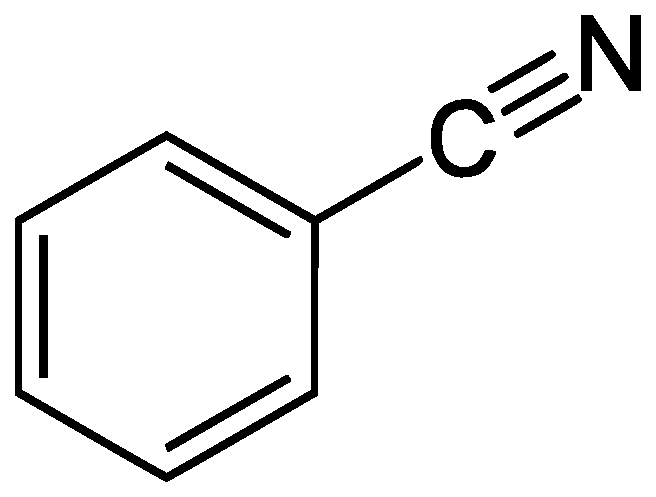
\includegraphics[width =0.7\textwidth]{Bilder/Grundlagen/Benzonitrile_structure.pdf}      
        \caption{Benzonitrile}
      \label{fig:BN}
    \end{subfigure}
    \hspace{\fill}
    \begin{subfigure}[b]{0.3\textwidth}
      \centering
      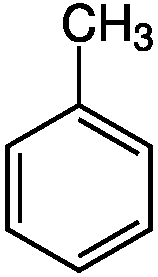
\includegraphics[width = 0.6\textwidth]{Bilder/Grundlagen/Toluen.pdf}      
      \caption{Toluen}
      \label{fig:Tol}
    \end{subfigure}
    \caption{Solvents used in this lab practice}
    \label{fig:Solvents}
\end{figure}

Benzonitrile is a colorless solvent with a sweet bitter almond odour. As a solvent it show a high polarity compared to toluene due to its C -- N bound. 
Both solvents have the characteristic benzene ring. Since they are not green solvents and can cause cancer, these two solvents are replaced in industry whenever possible. 

\subsection{ZnTPP and ZnOEP}
\label{subsec:ZnTPPZnOEP}

In the following section ZnTPP and ZnOEP are introduced.



\begin{figure}[h]
    \centering
    \begin{subfigure}[b]{0.5\textwidth}
        \centering
        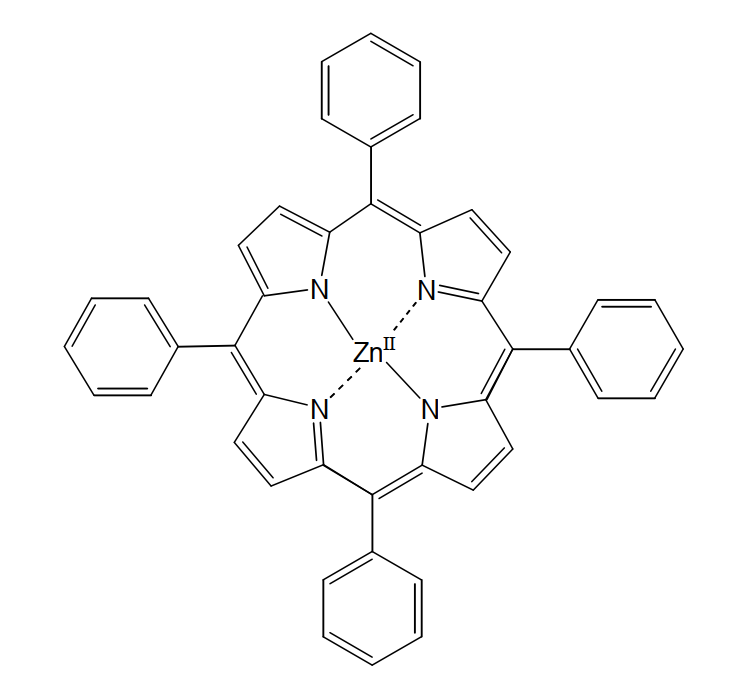
\includegraphics[width =0.7\textwidth]{Bilder/Grundlagen/ZnTPP.png}      
        \caption{5,10,15,20-Tetraphenyl-21H,23H-porphinzink(II) \newline M = 678,11 g/mol}
      \label{fig:BN}
    \end{subfigure}
    \hspace{\fill}
    \begin{subfigure}[b]{0.3\textwidth}
      \centering
      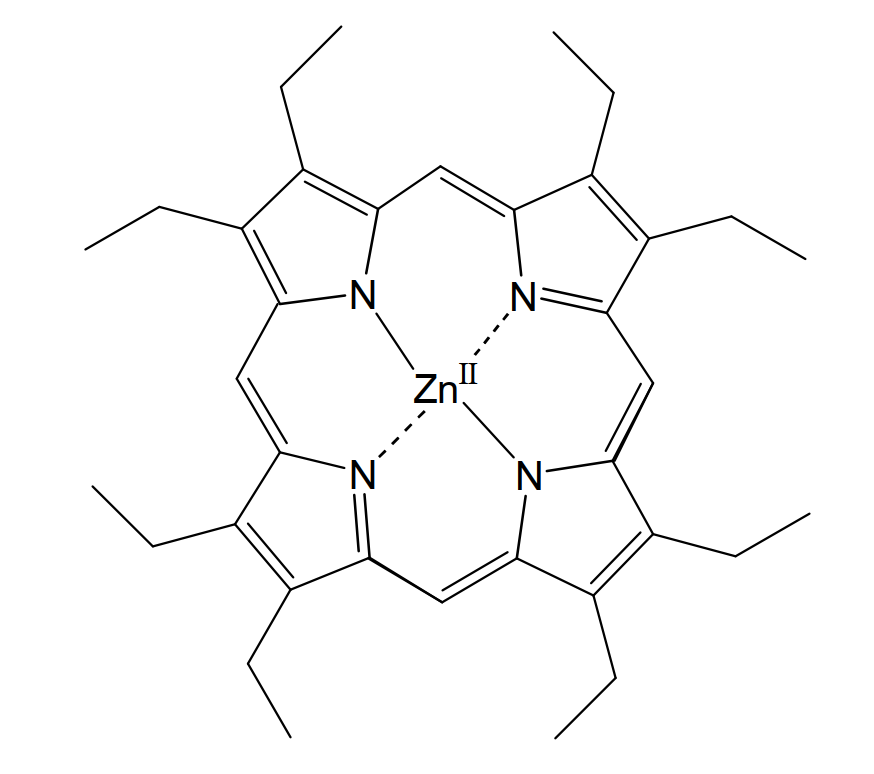
\includegraphics[width = 0.6\textwidth]{Bilder/Grundlagen/ZnOEP.png}      
      \caption{2,3,7,8,12,13,17,18-Octaethyl-21H,23H-porphinzink(II), M = 598,15 g/mol}
      \label{fig:Tol}
    \end{subfigure}
    \caption{Solvents used in this lab practice}
    \label{fig:Solvents}
\end{figure}
